% !TeX spellcheck = cs_CZ
%{\tikzset{external/prefix={tikz/FYZI/}}
% \tikzset{external/figure name/.add={ch21_}{}}
%=========================== Kapitola: Harmonický oscilátor ========================================
\setchaptertoc
\chapter{Harmonický oscilátor}\label{fyz:IchapXXI}

  \section{Lineární diferenciální rovnice}\label{fyz:IchapXXIsecI}
  \section{Harmonický oscilátor}\label{fyz:IchapXXIsecII}
  \section{Harmonický pohyb a pohyb po kružnici}\label{fyz:IchapXXIsecIII}
  \section{Počáteční podmínky}\label{fyz:IchapXXIsecIV}
  \section{Nucené kmity}\label{fyz:IchapXXIsecV}
  \section{Příklady a cvičení}\label{fyz:IchapXXIsecVI}

    \begin{figure}[ht!] %\ref{fyz:fig246}
      \centering
      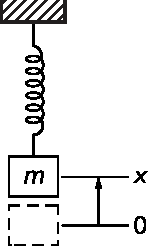
\includegraphics[width=0.3\linewidth]{fyz_fig246.pdf}
      \caption{Těleso upevněné na pružině - jednoduchý příklad harmonického oscilátoru
               (\cite[s.~287]{Feynman01})}
      \label{fyz:fig246}
    \end{figure}

    \begin{figure}[ht!] %\ref{fyz:fig247}
      \centering
      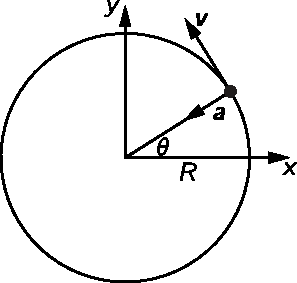
\includegraphics[width=0.5\linewidth]{fyz_fig247.pdf}
      \caption{Částice pohybující se po kruhové dráze konstantní rychlostí
               (\cite[s.~290]{Feynman01})}
      \label{fyz:fig247}
    \end{figure}

    \begin{figure}[ht!] %\ref{fyz:fig248}
      \centering
      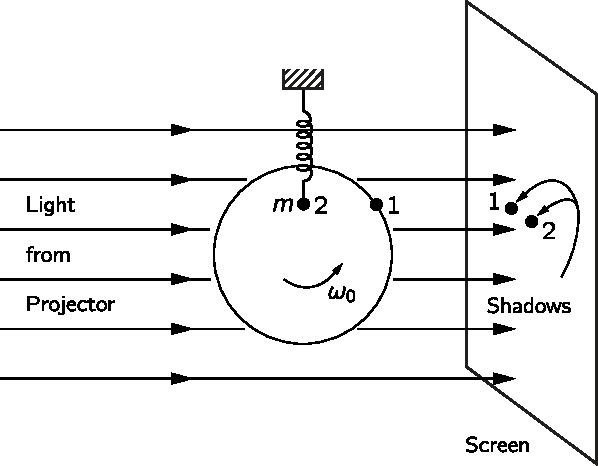
\includegraphics[width=0.5\linewidth]{fyz_fig248.pdf}
      \caption{Demonstrace ekvivalence jednoduchého harmonického pohybu a rovnoměrného pohybu po 
               krunici
               (\cite[s.~290]{Feynman01})}
      \label{fyz:fig248}
    \end{figure}

    \todo[inline]{Kapitola fey1ch21 je zcela prázdná, pouze obrázky}   
%} %tikzset
%---------------------------------------------------------------------------------------------------